\documentclass[9pt]{beamer}
\usepackage{kotex}
\usepackage{amsfonts,amssymb,amsthm}
\usepackage[dvipsnames]{xcolor}
\usepackage{xcolor}
\usepackage{etoolbox}
\usepackage{braket}
\usepackage{qcircuit}

%## color
\definecolor{customBlack}{HTML}{3B4252}
\definecolor{customBlackGrey}{HTML}{434C5e}
\definecolor{cuatomGrey}{HTML}{4C566A} 
\definecolor{customWhite}{HTML}{ECEFF4} 
\definecolor{customBlue}{HTML}{6082B6}  
\definecolor{customRed}{HTML}{BF616A}
\definecolor{vividauburn}{rgb}{0.58, 0.15, 0.14}


%## Theme & custom
% \usetheme{metropolis}           % Use metropolis theme
% \metroset{block=fill}
\usetheme{moloch} % modern fork of the metropolis theme
\molochset{block=fill}
\setbeamersize{text margin left=5mm, text margin right=5mm}
\setbeamercolor{palette primary}{bg=customBlack}
\setbeamercolor{alerted text}{fg=customRed}
\setbeamercolor{itemize item}{fg=customBlue}
\setbeamercolor{enumerate item}{fg=customBlue}


%## font
\usefonttheme[onlymath]{serif}
% \setbeamerfont{normal text}{size=\small}
% \setbeamerfont{math text}{size=\tiny}


%## Theorem title, numbering
\makeatletter
\setbeamertemplate{theorem begin}
{%
\begin{\inserttheoremblockenv}
{%
\inserttheoremheadfont
\inserttheoremname
\ifx\inserttheoremaddition\@empty\else\ of\ \inserttheoremaddition\fi%
\inserttheorempunctuation
}%
}
\setbeamertemplate{theorem end}{\end{\inserttheoremblockenv}}
\makeatother
\setbeamertemplate{theorems}[numbered]  


%## Custom block
\setbeamercolor{block title}{bg=customBlue, fg=white}
\setbeamercolor{block body}{bg=customWhite, fg=customBlack}
\setbeamercolor{block title alerted}{%
    use={block title, alerted text},
    bg=customRed,
    fg=white
}
\setbeamercolor{block body alerted}{%
    use={block title, alerted text},
    bg=customWhite,
    fg=customBlack
}
\AtBeginEnvironment{definition}{%
    \setbeamercolor{block title}{fg=white,bg=customBlackGrey}
    \setbeamercolor{block body}{fg=customBlack, bg=customWhite}
}
\AtBeginEnvironment{theorem}{%
    \setbeamercolor{block title}{fg=white,bg=customBlackGrey}
    \setbeamercolor{block body}{fg=customBlack, bg=customWhite}
}
\AtBeginEnvironment{corollary}{%
    \setbeamercolor{block title}{fg=white,bg=customBlackGrey}
    \setbeamercolor{block body}{fg=customBlack, bg=customWhite}
}
\AtBeginEnvironment{lemma}{%
    \setbeamercolor{block title}{fg=white,bg=customBlackGrey}
    \setbeamercolor{block body}{fg=customBlack, bg=customWhite}
}


%! Useful command
\renewcommand{\Pr}{\text{Pr}}
% $\ast$ \underline{Proof}:
%\checkmark \underline{meaning}:

\title{4. Basics of Quantum Computer}
\date{\today}
\author{Vaughan Sohn}
% \institute{Centre for Modern Beamer Themes}


\begin{document}
    %#################################### 
    \maketitle
    
    %#################################### 
    \begin{frame}
        \frametitle{Contents}
        \tableofcontents
    \end{frame}


    %#################################### 
    \begin{section}{Quantum Circuit model}
        \begin{frame}
            \frametitle{Component of quantum circuit model}
            \begin{itemize}
                \item Classical computer를 표현하기 위해서 circuit model을 사용한 것 처럼, quantum computer를 표현하기 위한 circuit model을 설계할 수 있다.
                \item Quantum circuit은 정보의 단위로 \textit{qubit}를 사용하며, logic gate와 같이 간단한 연산을 수행하는 quantum gate를 이용한다.
                \item Qubit와 quantum gate는 다음과 같은 특징을 가진다.
                    \begin{itemize}
                        \item Qubit는 superposition, entanglement와 같은 특징을 가진다.
                        \item Quantum gate는 input과 output qubit의 개수가 동일한 \textit{unitary operator}여야 한다.
                    \end{itemize}
                    
                \item Quantum circuit은 다음과 같이 나타낸다. Operation 순서는 left to right, qubit의 나열순서는 top to bottom이다.
                $\Rightarrow$ Matrix-vector 표기법과의 순서를 혼동하지 않도록 주의하자.
                $$\ket{\psi} = C(X)C(X)U\ket{q_0q_1q_2q_3}$$
                
                \vspace{-0.5cm}
                \begin{table}[h]
                    \[
                    \begin{array}{c}
                    \Qcircuit @C=1.5em @R=.8em {
                        \lstick{\ket{q_0}} & \ctrl{2} & \targ & \gate{U} & \qw \\
                        \lstick{\ket{q_1}} & \qw & \ctrl{-1} & \qw & \qw \\
                        \lstick{\ket{q_2}} & \targ & \ctrl{-1} & \ctrl{-2} & \qw \\
                        \lstick{\ket{q_3}} & \qw & \ctrl{-1} & \qw & \qw
                    }
                    \end{array}
                    \]
                    \caption{Quantum Circuit} \label{fig:ex_qc} 
                \end{table}

            \end{itemize}
        
        \end{frame}

        \begin{frame}
            \frametitle{Qubit}
            \begin{itemize}
                \item Computational basis $\{ket 0, \ket 1\}$에 대하여 single qubit은 다음과 같이 표현한다.
                $$ \begin{aligned} \ket \psi &= a \ket 0 + b \ket 1  \\  &= e^{i\alpha} \left( \cos \frac{\theta}{2} \ket 0 + e^{i \varphi} \sin \frac{\theta}{2}  \ket 1 \right) \\&= \cos\frac{\theta}{2} \ket 0 + e^{i \varphi} \sin\frac{\theta}{2} \ket 1\end{aligned}$$ 
                \item Bloch sphere를 이용하여 2개의 parameter $(\theta, \phi)$에 대해 qubit을 나타낼 수 있다.
                $$\ket{\psi} = (\sin \theta \cos \varphi,\ \sin \theta \sin \varphi,\ \cos \theta)$$
            \end{itemize}    
            \begin{columns}
                \begin{column}{0.65\textwidth}
                    \begin{figure}
                        \centering
                        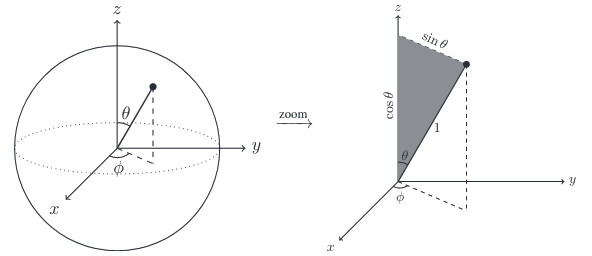
\includegraphics[width=0.95\columnwidth]{image/L4_bloch_1.png}
                    \end{figure}
                \end{column}
                \begin{column}{0.35\textwidth}
                    
                    \begin{figure}
                        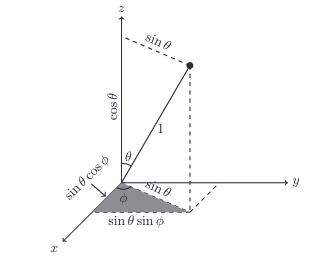
\includegraphics[width=0.9\columnwidth]{image/L4_bloch_2.png}
                    \end{figure}
                \end{column}
            \end{columns}
        \end{frame}
        
    \end{section}

    %#################################### 
    \begin{section}{Quantum Gates}
        \begin{frame}
            \frametitle{Single-qubit gate}
                \begin{itemize}
                    \item Pauli operator:
                    $$
                    X \equiv\left(\begin{array}{cc}
                    0 & 1 \\
                    1 & 0
                    \end{array}\right) ; \quad Y \equiv\left(\begin{array}{cc}
                    0 & -i \\
                    i & 0
                    \end{array}\right); \quad Z \equiv\left(\begin{array}{cc}
                    1 & 0 \\
                    0 & -1
                    \end{array}\right)
                    $$
                    \item Hadamard, Phase, $\pi/8$ gate [$\ast$]:
                    $$
                    H=\frac{1}{\sqrt{2}}\left(\begin{array}{cc}
                    1 & 1 \\
                    1 & -1
                    \end{array}\right) ; \quad S=\left(\begin{array}{ll}
                    1 & 0 \\
                    0 & i
                    \end{array}\right); \quad T=\left(\begin{array}{cc}
                    1 & 0 \\
                    0 & \exp (i \pi / 4)
                    \end{array}\right) .
                    $$
                \end{itemize}
                \vspace{0.4cm}
                $\Rightarrow$
                \vspace{0.6cm}
                $$T = \qquad \qquad \qquad \qquad \qquad \qquad \qquad \qquad \qquad \qquad \qquad \qquad \qquad $$
                \vspace{1.2cm}
        \end{frame}

        \begin{frame}
            \frametitle{Single-qubit gate}
                \begin{itemize}
                    \item Rotation operator:
                    $$
                    \begin{aligned}
                    & R_x(\theta) \equiv e^{-i \theta X / 2}=\cos \frac{\theta}{2} I-i \sin \frac{\theta}{2} X=\left(\begin{array}{cc}
                    \cos \frac{\theta}{2} & -i \sin \frac{\theta}{2} \\
                    -i \sin \frac{\theta}{2} & \cos \frac{\theta}{2}
                    \end{array}\right) \\
                    & R_y(\theta) \equiv e^{-i \theta Y / 2}=\cos \frac{\theta}{2} I-i \sin \frac{\theta}{2} Y=\left(\begin{array}{cc}
                    \cos \frac{\theta}{2} & -\sin \frac{\theta}{2} \\
                    \sin \frac{\theta}{2} & \cos \frac{\theta}{2}
                    \end{array}\right) \\
                    & R_z(\theta) \equiv e^{-i \theta Z / 2}=\cos \frac{\theta}{2} I-i \sin \frac{\theta}{2} Z=\left(\begin{array}{cc}
                    e^{-i \theta / 2} & 0 \\
                    0 & e^{i \theta / 2}
                    \end{array}\right )
                    \end{aligned}
                    $$
                    \item \textit{Generalized} rotation operator:
                    \\$\hat n = (n_x, n_y, n_z)$를 기준으로 $\theta$만큼 회전을 수행하는 rotation gate.
                    $$
                    R_{\hat{n}}(\theta) \equiv \exp (-i \theta \hat{n} \cdot \vec{\sigma} / 2)=\cos \left(\frac{\theta}{2}\right) I-i \sin \left(\frac{\theta}{2}\right)\left(n_x X+n_y Y+n_z Z\right)
                    $$
                    \begin{alertblock}{Rotation operator}
                        Rotation operator가 중요한 이유는 서로 다른 두 axis에 대한 rotation operator가 존재한다면, single qubit unitary gate를 decomposition할 수 있기 때문이다!
                    \end{alertblock}
                \end{itemize}
        \end{frame}


        \begin{frame}
            \frametitle{Single-qubit gate decomposition}
                \begin{theorem}[ZY decomposition]
                    Suppose $U$ is a unitary operation on a single qubit. Then there exist real numbers $\alpha, \beta, \gamma$ and $\delta$ such that,
                    $$U=e^{i \alpha} R_z(\beta) R_y(\gamma) R_z(\delta)$$
                \end{theorem}\label{thr:ZY-de}
                
                \begin{theorem}
                    Suppose $U$ is a unitary gate on a single qubit. Then there exist unitary operators $A, B, C$ on a single qubit such that $ABC = I$ and
                    $$ U = e^{i\alpha} AXBXC $$
                    where $\alpha$ is some overall phase factor and $X$ is a Pauli-X operator.
                \end{theorem}\label{thr:Pauli-de}
                \vspace{0.2cm}
                \checkmark \underline{meaning}: 어떤 single-qubit unitary gate이던지 rotation operator decomposition을 활용하면 arbitrary single qubit gate 3개와 Pauli-X gate로 나타낼 수 있다.

        \end{frame}

        \begin{frame}
            \frametitle{Single-qubit gate decomposition}
                $\ast$ \underline{Proof}:
                \\Theorem \ref{thr:ZY-de}를 이용하면, single qubit gate $A, B, C$를 rotation gate로 decomposition 할 수 있다. 각 gate가 다음과 같이 decomposition 된다고 하자.
                \begin{itemize}
                    \item $A \triangleq R_z(\beta)R_y\left( \frac{\gamma}{2} \right)$
                    \item $B \triangleq R_y\left( -\frac{\gamma}{2} \right)R_z\left( -\frac{\delta + \beta}{2} \right)$
                    \item $C \triangleq R_Z\left(\frac{\delta-\beta}{2} \right)$
                \end{itemize}
                \vspace{0.8cm}
                $$ABC = \qquad \qquad \qquad \qquad \qquad \qquad \qquad \qquad \qquad \qquad $$
                \vspace{0.4cm}
                $$XBX = \qquad \qquad \qquad \qquad \qquad \qquad \qquad \qquad \qquad \qquad $$
                \vspace{0.4cm}
                $$AXBXC = \qquad \qquad \qquad \qquad \qquad \qquad \qquad \qquad \qquad \qquad $$
        \end{frame}

        \begin{frame}
            \frametitle{Controlled gate}
            \vspace{0.5cm}
            \begin{itemize}
                \item Controlled gate는 기본적으로 2-qubit gate이다.
                \item Control qubit의 값에 따라서, target qubit에 대한 operator $U$의 적용 유무가 결정된다. (일반적으로 $\ket 1$이면 적용한다는 의미)
                $$ C(U)\ket{ct} = \begin{cases} U\ket{ct} & \text{if } \ket c = \ket 1 \\ \ket{ct} & \text{if } \ket c = \ket 0 \end{cases}$$
                \item Control qubit의 spectral decomposition은 다음과 같다.
                \vspace{0.1cm}
                $$C(U) = \ket 0 \bra 0 \otimes I + \ket 1 \bra 1 \otimes U$$
                \vspace{0.3cm}
                \item Gate symbol:
                \begin{itemize}
                    \item 점이 있는 곳이 control qubit이고 gate symbol이 있는 곳이 target qubit이다.
                    \vspace{0.1cm}
                    \item Target qubit이 검은색이면 $\ket 1$일 때 동작함을 의미하고, 만약 속이 채워지지 않은 점이라면 $\ket 0$일 때 동작함을 의미한다.
                \end{itemize} 
            \end{itemize}
            \vspace{-0.2cm}
            
            \begin{table}[h]
            \[
            \begin{array}{c}
            \Qcircuit @C=1.5em @R=.8em {
                \lstick{\ket{c}} & \ctrl{1} & \qw \\    
                \lstick{\ket{t}} & \gate{U} & \qw     
            }
            \end{array}
            \]
            \caption{Controlled-U gate} \label{fig:cu} 
            \end{table}
            
        \end{frame}

        \begin{frame}
            \frametitle{Controlled NOT gate}
            \vspace{0.4cm}
                \begin{itemize}
                    \item 어떤 unitary gate이든지 controlled gate로 사용될 수 있지만, Pauli $X$ gate에 대한 controlled gate인 CNOT gate가 특히나 더 중요하다.
                    \item CNOT gate는 control qubit가 $\ket 1$일 때, target qubit의 값을 반전시킨다. 마치 XOR gate처럼 동작하기 때문에, CNOT gate를 다음과 같이 표현한다.
                    \begin{columns}
                        \begin{column}{0.4\textwidth}
                            \vspace{-0.4cm}
                            \begin{align*} C(X)\ket{00} = \ket{00} \\ C(X)\ket{01} = \ket{01} \\ C(X)\ket{10} = \ket{11} \\ C(X)\ket{11} = \ket{10} \end{align*}
                        \end{column}
                        \begin{column}{0.6\textwidth}
                            \vspace{0.4cm}
                            $$ C(X)\ket{ct} = \ket{c}\ket{t \oplus c}$$
                            \vspace{-1cm}
                            \begin{table}[h]
                            \[
                            \begin{array}{c}
                            \Qcircuit @C=1.5em @R=.8em {
                                \lstick{\ket{c}} & \ctrl{1} & \qw \\    
                                \lstick{\ket{t}} & \targ & \qw     
                            }
                            \end{array}
                            \]
                            \caption{Controlled NOT gate} \label{fig:cnot} 
                            \end{table}
                        \end{column}
                    \end{columns}

                    \item CNOT gate를 사용하면 \alert{entangled state}를 만들 수 있다.
                    \begin{enumerate}
                        \item initial state: $\ket{00}$
                        \item after $H$ gate: $(H \otimes I) \ket{00} = \frac{\ket 0 + \ket 1}{\sqrt 2} \ket 0$
                        \item after $C(X)$ gate: $C(X) \frac{\ket 0 + \ket 1}{\sqrt 2} \ket 0 = \frac{\ket{00} + \ket{11}}{\sqrt 2}$ $\rightarrow$ \textit{Bell state!}
                    \end{enumerate}
                    \begin{table}[h]
                    \[
                    \begin{array}{c}
                    \Qcircuit @C=1.5em @R=.8em {
                        \lstick{\ket{0}} & \gate{H} & \ctrl{1} & \qw \\    
                        \lstick{\ket{0}} & \qw & \targ & \qw     
                    }
                    \end{array}
                    \]
                    \end{table}
                \end{itemize}
        \end{frame}

        \begin{frame}
            \frametitle{Controlled gate decomposition}
                Theorem \ref{thr:Pauli-de}를 이용하면, CNOT gate를 다음과 같이 3개의 single-qubit unitary operation $A,B,C$와 Controlled-$X$ gate 2개를 사용하여 decomposition할 수 있다.
                \vspace{0.2cm}
                $$C(U) = e^{i\alpha} AC(X)BC(X)C$$
                \vspace{-1.2cm}
                \begin{columns}
                    \begin{column}{0.3\textwidth}
                        \begin{table}[h]
                            \[
                            \begin{array}{c}
                            \Qcircuit @C=1.5em @R=.8em {
                                \lstick{\ket{c}} & \ctrl{1} & \qw \\    
                                \lstick{\ket{t}} & \gate{U} & \qw     
                            }
                            \end{array}
                            \]
                        \end{table}
                    \end{column}
                    \begin{column}{0.1\textwidth}
                        \\$=$
                    \end{column}
                    \begin{column}{0.6\textwidth}
                        \begin{table}[h]
                            \[
                            \begin{array}{c}
                            \Qcircuit @C=1.5em @R=.8em {
                                \lstick{\ket{c}} & \qw      & \ctrl{1} & \qw        &\ctrl{1}   &\gate{\begin{pmatrix} 1 & 0 \\ 0 & e^{i\alpha} \end{pmatrix}} &\qw\\    
                                \lstick{\ket{t}} & \gate{C} & \targ    & \gate{B}   &\targ      & \gate{A} &\qw
                            }
                            \end{array}
                            \]
                        \end{table}
                    \end{column}
                \end{columns}
                \vspace{-0.5 cm}
                \begin{columns}
                    \begin{column}{0.3\textwidth}
                        \begin{align*} C(U)\ket{00} &= \ket{00} \\ C(U)\ket{01} &= \ket{01} \\ C(U)\ket{10} &= \ket{1}U\ket{0} \\ C(U)\ket{11} &= \ket{1}U\ket{1}\end{align*}
                    \end{column}
                    \begin{column}{0.05\textwidth}
                        \\$=$
                    \end{column}
                    \begin{column}{0.65\textwidth}
                        \centering
                        \begin{itemize}
                            \item If $\ket{c} = \ket{0}$:
                            $$ \xrightarrow{I\otimes C}  \ket{0}C\ket{t} \xrightarrow{C(X)} \ket{0}C\ket{t} \xrightarrow{I\otimes B} \ket{0}BC\ket{t}$$
                            $$ \xrightarrow{C(X)}  \ket{0}BC\ket{t}   \xrightarrow{I\otimes A} \ket{0}ABC\ket{t}$$
                            \item If $\ket{c} = \ket{1}$:
                            $$ \xrightarrow{I\otimes C}  \ket{1}C\ket{t} \xrightarrow{C(X)} \ket{1}XC\ket{ t} \xrightarrow{I\otimes B} \ket{1}BXC\ket{ t}$$
                            $$ \xrightarrow{C(X)}  \ket{1}XBXC\ket{t}   \xrightarrow{I\otimes A} \ket{1}AXBXC\ket{t}$$
                        \end{itemize}
                    \end{column}
                \end{columns}
        
        \end{frame}
        \begin{frame}
            \frametitle{Controlled gate on multiple-qubit}
                (generalize) $n+k$개의 qubit에 대해, $n$개가 control qubit이고 $k$개가 target qubit; 즉 $U$가 $k$-qubit에 대한 operator인 controlled gate는 다음과 같이 정의한다. 
                $$C^n(U) \ket{c_1c_2 \cdots c_n}\ket{t}= \ket{c_1c_2 \cdots c_n} U^{\prod_{i} c_i}\ket{t}$$
                $\Rightarrow$ control qubit들이 모두 1이면 $U$ operator가 적용되고, 그렇지 않으면 아무것도 수행하지 않는다.
                \vspace{0.5cm}
                \\ \textbf{Example} $n=4, t=3$ controlled gate
                \vspace{-0.3cm}
                \begin{table}[h]
                    \[
                    \begin{array}{c}
                    \Qcircuit @C=1.6em @R=.9em {
                        \lstick{\ket{c_1}} & \ctrl{4} & \qw \\    
                        \lstick{\ket{c_2}} & \ctrl{3} & \qw \\    
                        \lstick{\ket{c_3}} & \ctrl{2} & \qw \\    
                        \lstick{\ket{c_4}} & \ctrl{1} & \qw  
                        \inputgroupv{5}{7}{.9em}{1.7em}{\ket{t}}\\
                        \lstick{} & \multigate{2}{U} & \qw   \\
                        \lstick{} &  \ghost{U} & \qw   \\
                        \lstick{} &  \ghost{U} & \qw   \\
                    }
                    \end{array}
                    \]
                \end{table}
        
        \end{frame}
        \begin{frame}
            \frametitle{Controlled gate on multiple-qubit decomposition}
            \textbf{Decomposition of $C^2(U)$}
            \\Control qubit이 2개인 unitary gate는  $V^2 = U$를 만족하는 unitary gate $V$에 대해서 다음과 같이 decomposition 할 수 있다.
                \vspace{-0.5cm}
                \begin{columns}
                    \begin{column}{0.3\textwidth}
                        \begin{table}[h]
                            \[
                            \begin{array}{c}
                            \Qcircuit @C=1.5em @R=1.1em {
                                \lstick{\ket{c_1}} & \ctrl{2} & \qw \\    
                                \lstick{\ket{c_2}} & \ctrl{1} & \qw \\    
                                \lstick{\ket{t}} & \gate{U} & \qw     
                            }
                            \end{array}
                            \]
                        \end{table}
                    \end{column}
                    \begin{column}{0.1\textwidth}
                        \\$=$
                    \end{column}
                    \begin{column}{0.6\textwidth}
                        \begin{table}[h]
                            \[
                            \begin{array}{c}
                                \Qcircuit @C=1.5em @R=1.1em {
                                \lstick{\ket{c_1}}  & \qw       & \ctrl{1}  & \qw               & \ctrl{1}  & \ctrl{2}  & \qw   \\    
                                \lstick{\ket{c_2}}  & \ctrl{1}  & \targ     & \ctrl{1}          & \targ     & \qw       & \qw   \\    
                                \lstick{\ket{t}}    & \gate{V}  & \qw       & \gate{V^\dagger}  & \qw       & \gate{V}  & \qw
                            }
                            \end{array}
                            \]
                        \end{table}
                    \end{column}
                \end{columns}
                \vspace{0.2cm}
                $\ast$ \underline{Proof}: 위와 같이 decomposition한 gate가 실제로 $C^2(U)$와 동일하게 동작하는지 확인해보자.
                \\ $\Rightarrow$
                \vspace{2cm}
        \end{frame}

        \begin{frame}
            \frametitle{Controlled gate on multiple-qubit decomposition}
            (generalize) Control qubit이 $n$개인 unitary gate는 Toffoli gate ($C^2(X)$)를 이용하여 다음과 같이 구현한다. 구현을 위해서 $n-1$개의 ancilla qubit을 필요로한다.
            \begin{table}[h]
                \[
                \begin{array}{c}
                    \Qcircuit @C=1.5em @R=1.1em {
                    \lstick{\ket{c_1}}  & \ctrl{5}  & \qw       &\qw    &\qw    &\qw&\qw&\qw&\qw&\ctrl{5}&\qw\\
                    \lstick{\ket{c_2}}  & \ctrl{4}  & \qw       &\qw    &\qw    &\qw&\qw&\qw&\qw&\ctrl{4}&\qw\\
                    \lstick{\ket{c_3}}  & \qw       & \ctrl{4}  &\qw    &\qw    &\qw &\qw&\qw&\ctrl{4}&\qw&\qw\\
                    \lstick{\ket{c_4}}  & \qw       & \qw       &\ctrl{4}&\qw   &\qw&\qw&\ctrl{4}&\qw&\qw&\qw\\
                    \lstick{\ket{c_5}}  & \qw       & \qw       &\qw    &\ctrl{4}&\qw&\ctrl{4}&\qw&\qw&\qw&\qw\\
                    \lstick{\ket{0}}    & \targ     & \ctrl{1}  &\qw    &\qw    &\qw &\qw &\qw &\ctrl{1}&\targ&\qw\\
                    \lstick{\ket{0}}    & \qw       & \targ     &\ctrl{1}&\qw   &\qw &\qw   &\ctrl{1} &\targ&\qw&\qw\\
                    \lstick{\ket{0}}    & \qw       & \qw       &\targ  &\ctrl{1}&\qw &\ctrl{1}&\targ&\qw&\qw&\qw\\
                    \lstick{\ket{0}}    & \qw       & \qw       &\qw    &\targ  &\ctrl{1}&\targ&\qw&\qw&\qw&\qw\\
                    \lstick{\ket{t}}    & \qw       & \qw       &\qw   &\qw     &\gate{U}&\qw&\qw&\qw&\qw&\qw\\
                }
                \end{array}
                \]
            \end{table}
        \end{frame}

        \begin{frame}
            \frametitle{Controlled gate on multiple-qubit decomposition}
                \textbf{Complexity}:
                \\ $C^n(U)$ gate를 구현하기 위해서는 다음과 같은 complexity를 가진다.
                \begin{itemize}
                    \item $n-1$개의 ancilla qubit
                    \item $2(n-1)$개의 Toffoli gate 
                    \begin{itemize}
                        \item $4(n-1)$개의 CNOT gate
                        \item $6(n-1)$개의 single unitary gate
                    \end{itemize}
                    $$O(n) $$
                \end{itemize}
                
                \vspace{0.4cm}
                $\ast$ \underline{Proof}:$2(n-1)$개의 Toffoli gate, 그리고 $C(U)$ gate를 사용하여 decomposition한 회로가 왜 $C^n(U)$와 동일하게 동작하는지 분석해보자.
                \\ $\Rightarrow$
                \vspace{2cm}
        \end{frame}

        \begin{frame}
            \frametitle{Summary}
            \begin{block}{Summary}
                \begin{itemize}
                    \item  Quantum circuit을 구성하는 다양한 gate들을 소개한다.
                    \item  Single qubit gate는 다음과 equivalent하다.
                    \begin{itemize}
                        \item 두 가지 axis에 대한 rotation gates
                        \item single qubit gates와 Pauli-X gates
                    \end{itemize}
                    
                    \item  Single qubit controlled gate = single qubit gates and CNOT gates
                    \item  Multiple-qubit controlled gate = \textit{single qubit controlled gates} and CNOT gates
                    \\ $\rightarrow$ \textit{single qubit gates and CNOT gates}
                    
                \end{itemize}
            \end{block}
            \vspace{0.2cm}
            \textit{Some remarks}
            \begin{itemize}
                \item control qubit이 $\ket 0$일 때 동작하는 controlled gate의 구현은 다음과 같다.
                $$ XC(U)X = C'(U) $$
                \item (symbol) single-qubit gate가 여러개의 target qubit에 적용되는 경우:
                \vspace{-0.2cm}
                \begin{table}[h]
                    \[
                    \begin{array}{c}
                        \Qcircuit @C=1.5em @R=1.1em {
                        \lstick{\ket{c}}  &\ctrl{2}  & \qw   \\    
                        \lstick{\ket{t_1}}&\targ    & \qw   \\    
                        \lstick{\ket{t_2}}&\targ    & \qw   \\    
                    }
                    \end{array}
                    \]
                \end{table}
                
            \end{itemize}
            
        
        \end{frame}

    \end{section}
    % 이 section에서는 single qubit gate, controlled gate를 decomposition하는 법을 배웠다.
    %! 이제 multiple qubit gate를 구현할 수만 있으면 quantum circuit을 구현할 수 있다!

    %#################################### 
    \begin{section}{Universial Quantum gate set: \{CNOT, single qubit gates\}}
        \begin{frame}
            \frametitle{Decomposition from n-qubit unitary gate to two-level unitary gates}
            \begin{theorem}\label{thr:two-level de}
                Unitary operator $U$ which acts on a $d$-dimensional Hilbert space ($d = 2^n$) may be decomposed into a product of \alert{two-level unitary matrices};
            \end{theorem}
            \vspace{0.2cm}
            \textbf{Two-level unitary:}
            \begin{itemize}
                \item $d$차원 Hilbert space의 벡터에 대해서 \alert{2개의} 벡터요소에만 작용
                \item $d\times d$ matrix에서 대부분은 identity matrix이고 자신이 작용하는 state에 대응되는 부분에만 항등행렬이 아닌 $2\times 2$ 행렬이 위치한다. 
                $$\begin{pmatrix} u_{11} & u_{12} & 0 \\ u_{22} & u_{22} & 0 \\ 0 & 0 & 1  \end{pmatrix} \quad  \text{ or } \quad \begin{pmatrix} u_{11} & 0  & u_{12} \\ 0 & 1 & 0 \\ u_{21} & 0 & u_{22}  \end{pmatrix}$$ 
            \end{itemize}

            \vspace{0.4cm}
            $\ast$ \underline{Proof}: from $3\times 3$ example, $(d=3)$
            $3\times 3$ unitary $U$에 대하여, 다음을 만족하는 two-level matrices가 존재함을 보이자.
            $$ U_3U_2U_1 U = I \qquad \Leftrightarrow \qquad U_1^\dagger U_2^\dagger U_3^\dagger$$
            
            \textit{where} 
            $$
            U=\left[\begin{array}{lll}
            a & d & g \\
            b & e & h \\
            c & f & j
            \end{array}\right]
            $$
        \end{frame}
        \begin{frame}
            \frametitle{Decomposition from n-qubit unitary gate to two-level unitary gates}
                $\ast$ \underline{Proof}: (contd.)
                \begin{itemize}
                    \item $b$의 값에 따라서 다음과 같이 $U_1$를 가정하자.
                    $$ U_1 \equiv\left[\begin{array}{lll} 1 & 0 & 0 \\ 0 & 1 & 0 \\ 0 & 0 & 1 \end{array}\right](b=0),\qquad
                    U_1 \equiv\left[\begin{array}{ccc}
                    \frac{a^*}{\sqrt{|a|^2+|b|^2}} & \frac{b^*}{\sqrt{|a|^2+|b|^2}} & 0 \\
                    \frac{b}{\sqrt{|a|^2+|b|^2}} & \frac{-a}{\sqrt{|a|^2+|b|^2}} & 0 \\
                    0 & 0 & 1
                    \end{array}\right] (b \ne 0) $$
                    \item 이렇게 가정한 $U_1$를 $U$에 곱하면, $b=0$이 된다.
                    $$
                    U_1 U=\left[\begin{array}{ccc}
                    a^{\prime} & d^{\prime} & g^{\prime} \\
                    0 & e^{\prime} & h^{\prime} \\
                    c^{\prime} & f^{\prime} & j^{\prime}
                    \end{array}\right]
                    $$
                    \item $c'$의 값에 따라서 다음과 같이 $U_2$를 가정하자.
                    $$U_2 \equiv\left[\begin{array}{ccc} a^{\prime *} & 0 & 0 \\ 0 & 1 & 0 \\ 0 & 0 & 1 \end{array}\right] (c'=0), \quad U_2 \equiv\left[\begin{array}{ccc}
                        \frac{a^{\prime *}}{\sqrt{\left|a^{\prime}\right|^2+\left|c^{\prime}\right|^2}} & 0 & \frac{c^{\prime *}}{\sqrt{\left|a^{\prime}\right|^2+\left|c^{\prime}\right|^2}} \\
                        0 & 1 & 0 \\
                        \frac{c^{\prime}}{\sqrt{\left|a^{\prime}\right|^2+\left|c^{\prime}\right|^2}} & 0 & \frac{-a^{\prime}}{\sqrt{\left|a^{\prime}\right|^2+\left|c^{\prime}\right|^2}}
                        \end{array}\right](c'\ne 0)$$
                \end{itemize}        
        \end{frame}

        \begin{frame}
            \frametitle{Decomposition from n-qubit unitary gate to two-level unitary gates}
                $\ast$ \underline{Proof}: (contd.)
                \begin{itemize}
                    \item 이렇게 가정한 $U_2$를 $U_1U$에 곱하면, $c'=0$이 되고, $a'=1$이 된다. 이때, unitary matrix의 조건에 의해서 첫번째 row vector의 norm이 반드시 1이 되어야하므로 $d''=0, g''=0$이어야한다. [$\ast$]
                    $$
                    U_2 U_1 U=\left[\begin{array}{lll}
                        1 & d^{\prime \prime} & g^{\prime \prime} \\
                        0 & e^{\prime \prime} & h^{\prime \prime} \\
                        0 & f^{\prime \prime} & j^{\prime \prime}
                        \end{array}\right]=\left[\begin{array}{lll}
                            1 & 0 & 0 \\
                            0 & e^{\prime \prime} & h^{\prime \prime} \\
                            0 & f^{\prime \prime} & j^{\prime \prime}
                            \end{array}\right]
                    $$
                    \item 마지막으로 $U_3 = (U_2U_1U)^\dagger$로 가정하자.그럼 자명하게 다음을 만족하므로, $3\times 3$ unitary matrix를 3개의 two-level matrix의 multiplication으로 decomposition 할 수 있다.
                    $$U_3U_2U_1U = (U_2U_1U)^\dagger(U_2U_1U) = I$$
                    \item (generalize) $d\times d$ matrix에 대해서도 $u_{11}=1$이고 나머지 행과 열은 0인 행렬을 two-level matrix들을 곱하여; $U_1U_2 \cdots U_{d-1}U$ 얻을 수 있다. 그러고 나서, 나머지 $d-1\times d-1$ 부분 행렬이 $2\times2$ 부분 행렬이 될 때까지 이 절차를 반복하면, 임의의 $d\times d$ 유니타리 행렬을 다음과 같이 표현할 수 있다.$\Box$
                    $$ U= V_1 \cdots V_k, \qquad k \le (d-1) + (d-2) + \cdots + 1 = \frac{d(d-1)}{2}$$
                    \vspace{-0.7cm}
                \end{itemize}        
        \end{frame}

        \begin{frame}
            \frametitle{Two-level unitary gate is controlled-U gate}
                % quantum state에서 각 벡터요소는 거기에 대응되는 basis state가 있으니까
                \begin{itemize}
                    \item 2-level unitary matrix는 $n$ system 전체에 작용하는 gate이지만 특정 벡터요소에만 작용하며, 이는 특정 \alert{basis state}에 대해서만 작용한다고 생각할 수 있다. 
                    \item 예를 들어, 다음과 같은 2-level unitary matrix는 $\ket{10}, \ket{11}$ basis state에만 비자명하게 작용한다. $\ket{c} = \ket{1}$일 때 동작하는 controlled-$U$ gate로 생각할 수 있다.
                    $$ \begin{pmatrix} 1 & 0  & 0 & 0 \\ 0 & 1 & 0 & 0\\ 0 & 0 & u_{00} &  u_{01}  \\0 & 0 & u_{10} & u_{11} \\ \end{pmatrix}  =u_{00} \ket{10}\bra{10} + u_{01}\ket{10}\bra{11} +u_{10} \ket{11}\bra{10}+ u_{11} \ket{11}\bra{11} + I_{\perp}$$
                    \item 그러나 문제점은 다음과 같은 two-level unitary matrix도 존재한다는 것이다. 
                    $$ \begin{pmatrix} u_{00} & 0  & 0 & u_{01} \\ 0 & 1 & 0 & 0\\ 0 & 0 & 1 &  0 \\ u_{10} & 0 & 0 & u_{11} \\ \end{pmatrix}  =u_{00} \ket{00}\bra{00} + u_{01}\ket{00}\bra{11} +u_{10} \ket{11}\bra{00}+ u_{11} \ket{11}\bra{11} + I_{\perp}$$
                    \item Two-level unitary matrix가 작용하는 basis가 1bit의 값이 다르다면, 그 1bit를 target qubit으로 생각해서 controlled-$U$ gate로 표현할 수 있다.
                    \item 그러나, 1bit이상이 달라지게 되면 더이상 controlled-U gate로 생각할 수 없다.
                \end{itemize}
                
                
        
        \end{frame}

        \begin{frame}
            \frametitle{Decomposition from n-qubit controlled-U gate to \{CNOT gates, single-qubit\}}
            \framesubtitle{$\Rightarrow$ Single qubit and CNOT gates are universal!}
            \begin{alertblock}{Idea}
                Basis $\ket{s},\ket{t}, D_H(s, t) > 1$에 대한 작용을 basis $D_H(g_i, g_j) = 1$에 대한 작용들의 연속으로 생각하는 것이다.
                $$\ket{s} = \ket{g_1} \rightarrow \ket{g_2} \rightarrow \ket{g_3} \cdots \rightarrow \ket{g_{m-1}},\  D_H(\ket{g_{m-1}},\ket{t}) = 1$$
            \end{alertblock}
            예를 들어, $\ket s = \ket{101001}$이고 $\ket t =\ket{110011}$이면 다음과 같은 변환을 수행할 수 있다.
            $$
            \begin{aligned}
            s & = &101001 \\
            g_2 & = &101011 \\
            g_3 & = &100011 \\
            t & = &110011
            \end{aligned}
            $$
            \begin{theorem}\label{thr:CNOT-single de}
                $n$-qubit controlled-$U$ gate can be decomposed into a single qubit gate and CNOT gates;
            \end{theorem}
            \vspace{0.2cm}
            

        \end{frame}

        \begin{frame}
            \frametitle{Decomposition from n-qubit controlled-U gate to \{CNOT gates, single-qubit\}}
            \framesubtitle{$\Rightarrow$ Single qubit and CNOT gates are universal!}
                $\ast$ \underline{Proof}: 
                \begin{itemize}
                    \item $\ket{s}=\ket{g_1}, \ket{t}=\ket{g_m}$에 대해서 작용하는 two-level unitary matrix는 다음과 같다.
                    $$U = u_{00} \ket{g_1}\bra{g_1} + u_{01}\ket{g_1}\bra{g_m} +u_{10} \ket{g_m}\bra{g_1}+ u_{11} \ket{g_m}\bra{g_m} + \sum_{s'\ne g_1, g_m} \ket{s'} \bra {s'}$$
                    \item $\ket{g_1}$을 $\ket{g_2}$로 변환하는 operator는 다음과 같다. (특정 qubit의 값을 반전)
                    $$V_{12} = \ket{g_2}\bra{g_1} + \ket{g_1}\bra{g_2}+ \sum_{s'\ne g_1, g_2} \ket{s'} \bra {s'}$$
                    
                    \item 따라서 변환하면 다음과 같이 $\ket{g_2}, \ket{g_m}$에 대해서 작용하는 operator가 된다.
                    $$V_{12}^\dagger UV_{12} = u_{00} \ket{g_2}\bra{g_2} + u_{01}\ket{g_2}\bra{g_m} +u_{10} \ket{g_m}\bra{g_2}+ u_{11} \ket{g_m}\bra{g_m} + I_{\perp} $$
                    \item 이를 반복하면, $\ket{g_{m-1}}, \ket{g_m}$에 대한 변환을 수행하는 controlled-$U$ gate가 된다.
                    $$C^{n-1}(U) \triangleq V_{m-2,{m-1}} \cdots  V_{2,3} V_{1,2} U V^\dagger_{1,2} V^\dagger_{2,3} \cdots V^\dagger_{m-2,{m-1}} $$
                \end{itemize}
        \end{frame}

        \begin{frame}
            \frametitle{Decomposition from n-qubit controlled-U gate to \{CNOT gates, single-qubit\}}
            \framesubtitle{$\Rightarrow$ Single qubit and CNOT gates are universal!}
                $\ast$ \underline{Proof}: (contd.)
                \begin{itemize}
                    \item $C^{n-1}(U)$ gate에 다시 basis를 변환하는 operator를 가하면, 원래의 matrix와 동등하다는 것을 알 수 있다.
                    $$ \begin{aligned} &(V_{m-2,{m-1}} \cdots  V_{2,3} V_{1,2})^\dagger C^{n-1}(U) (V^\dagger_{1,2} V^\dagger_{2,3} \cdots V^\dagger_{m-2,{m-1}})^\dagger \\
                        &= (V_{m-2,{m-1}} \cdots V_{1,2})^\dagger (V_{m-2,{m-1}} \cdots V_{1,2}) U  (V^\dagger_{1,2} \cdots V^\dagger_{m-2,{m-1}})^\dagger (V^\dagger_{1,2} \cdots V^\dagger_{m-2,{m-1}} )\end{aligned}$$
                    \item 따라서, 다음의 과정을 거쳐서 two-level matrix를 구현할 수 있다.
                    \begin{enumerate}
                        \item basis 변환: $\ket{s} \rightarrow \ket{g_{m-1}}$
                        \item Controlled-U gate: $C^{n-1}(U)$
                        \item 원본 basis로 다시 변환: $\ket{g_{m-1}} \rightarrow \ket{s}$
                    \end{enumerate}
                    \vspace{-0.2cm}
                    \begin{table}[h]
                        \[
                        \begin{array}{c}
                            \Qcircuit @C=1.0em @R=1.1em {
                            &\multigate{4}{V_{1, 2}}  &\multigate{4}{\cdots}  &\multigate{4}{V_{m-2, m-1}} & \ctrl{4}   &\multigate{4}{V^\dagger_{m-2, m-1}} &\multigate{4}{\cdots}  &\multigate{4}{V^\dagger_{1, 2}} &\qw  \\
                            &\ghost{V_{1, 2}}         &\ghost{\cdots}         &\ghost{V_{m-2, m-1}}        & \ctrl{3}   &\ghost{V^\dagger_{m-2, m-1}}    &\ghost{\cdots}         &\ghost{V^\dagger_{1, 2}} &\qw  \\    
                            &\ghost{V_{1, 2}}         &\ghost{\cdots}         &\ghost{V_{m-2, m-1}}        & \ctrl{2}   &\ghost{V^\dagger_{m-2, m-1}}    &\ghost{\cdots}         &\ghost{V^\dagger_{1, 2}} &\qw\\
                            &\ghost{V_{1, 2}}         &\ghost{\cdots}         &\ghost{V_{m-2, m-1}}        & \ctrl{1}   &\ghost{V^\dagger_{m-2, m-1}}    &\ghost{\cdots}         &\ghost{V^\dagger_{1, 2}} & \qw \\    
                            &\ghost{V_{1, 2}}         &\ghost{\cdots}         &\ghost{V_{m-2, m-1}}        & \gate{\tilde{U}}&\ghost{V^\dagger_{m-2, m-1}}   &\ghost{\cdots}         &\ghost{V^\dagger_{1, 2}} & \qw\\
                        }
                        \end{array}
                        \]
                    \end{table}
                \end{itemize}
        \end{frame}

        \begin{frame}
            \frametitle{Decomposition from n-qubit controlled-U gate to \{CNOT gates, single-qubit\}}
            \framesubtitle{$\Rightarrow$ Single qubit and CNOT gates are universal!}
            \textbf{Example} 다음의 $8\times 8$ two-level unitary operator를 구현하는 회로를 설계하라.
            $$ U=\left[\begin{array}{llllllll}
                a &  0^{\otimes 6} & c \\
                0^{\otimes 6}  & I^{6\times 6} & 0^{\otimes 6}  \\
                b & 0^{\otimes 6}  & d
                \end{array}\right], \quad \tilde{U} = \begin{bmatrix} a & c \\ b & d\end{bmatrix}$$
            $\Rightarrow$
                \vspace{2.6cm}
            \begin{corollary}\label{col:universial-ver1}
                single qubit and CNOT gates together can be used to implement an \alert{arbitrary $n$-qubit unitary operation}.
            \end{corollary}
            $\ast$ \underline{Proof}: Combine theorem \ref{thr:two-level de} and \ref{thr:CNOT-single de}, we can easily proof this corollary.$\Box$
        \end{frame}

        \begin{frame}
            \frametitle{Circuit complexity}
            그렇다면, $n$-qubit arbitrary unitary operator를 구현하기 위해서 필요한 총 gate의 개수는 몇 개일까?
            \begin{itemize}
                \item $d\times d$ gate $\equiv$ 최대 $d(d-2)/2$개의 two-level gate
                $$O(d^2) = O(4^n)$$
                \item (each) two-level gate $\equiv$ 최대 $2(n-1) + 1$개의 controlled gate (\textit{basis change})
                $$O(n)$$
                \item (each) controlled gate $\equiv$ 최대 $2(n-1)$개의 Toffoli gate
                $$O(n)$$
            \end{itemize}
            $\Rightarrow$ 따라서 다음과 같은 circuit complexity를 가지고 CNOT gates, single-qubit gates를 이용하여 어떤 unitary gate도 구현할 수 있다!
            $$ O(4^n) \times O(n) \times O(n) = O(n^24^n)$$
            
        
        \end{frame}

        \begin{frame}
            \frametitle{Summary}
            \begin{block}{Summary}
                \begin{itemize}
                    \item $n$-qubit unitary = $O(4^n)$개의 two-level unitary gates.
                    \item $n$-qubit two-level unitary gate = $O(n)$개의 controlled gates.
                    \\(basis를 변환한 뒤, controlled-U gate를 취하고 다시 원래 basis로 변환한다.)
                    \item $n$-qubit controlled gate = $O(n)$개의 CNOT / single-qubit gates.
                    \item 따라서 총 $O(n^24^n)$의 복잡도로 universal gate set $\{CNOT, \text{single-qubit gate}\}$를 이용하여 어떤 quantum gate이든지 구현할 수 있다.
                \end{itemize}
            \end{block}
        
        \end{frame}
    \end{section}
    
    %#################################### 
    % rotation이랑 다르게 discrete gate들임
    \begin{section}{Universial Quantum Discrete gate set: \{CNOT, H, S, T\}}
        

        \begin{frame}
            \frametitle{Approximating quantum circuits via discrete gate set}
                \textbf{Problem}: Universal gate set $\{CNOT, \text{single-qubit gate}\}$을 사용하면 어떠한 quantum gate이든지 오류없이 구현할 수 있다. 하지만, single-qubit gates는 $\theta$에 따라서 continuos한 gate이기 때문에 이로인하여 noise에 큰 영향을 받게된다.
                \vspace{0.2cm}
                \\ $ \Rightarrow $ \textbf{Idea}: Discrete gate set $\{CNOT, H, S, T\}$을 사용하여 gate를 \alert{approximation}하여 구현하고자 한다.
                \vspace{0.5cm}
                \begin{definition}[approximation error]\label{def:error}
                    We define the \textbf{error} when $V$ is implemented instead of $U$ by
                    $$E(U,V) \triangleq \max_{\ket{\psi}} \|(U-V) \ket{\psi}\|$$
                    where the maximum is over all normalized quantum states $\ket{\psi}$ in the state space.
                \end{definition}
                \vspace{0.2cm}
                \checkmark \underline{meaning}: $U$를 $V$로 근사했을 때 발생하는 error중에서 가장 큰 값으로 정의한다.
            
        
        \end{frame}

        \begin{frame}
            \frametitle{Approximating quantum circuits via discrete gate set}
                \begin{definition}[variational distance]\label{def:vari-dist}
                    We detine the \textbf{variational distance} as 
                    $$VD(P_U(m), P_V(m)) = \frac{1}{2} |P_U(m) - P_V(m)|,$$
                    and total variational distance 
                    $$TVD(P_U, P_V) = \frac{1}{2} \sum_m |P_U(m) - P_V(m) |,$$
                    where 
                    $$P_U (m) = \text{tr}[E_m U\ket \psi \bra \psi U^\dagger],\quad P_V (m) = \text{tr}[E_m V\ket \psi \bra \psi V^\dagger].$$
                \end{definition}
                \vspace{0.2cm}
                \checkmark \underline{meaning}: 각 gate $U, V$를 $\ket{\psi}$에 가한 뒤 관측했을 때, 그 outcome이 $m$일 확률이 $P_U(m), P_V(m)$이다. 두 probability distribution의 차이로 variational distance를 정의한다. 만약 두 분포가 거의 유사하다면, 두 unitary $U, V$를 구분하기 어려울 것이다. 
                \vspace{0.2cm}
                \begin{corollary}
                    If $E(U, V) < \epsilon$ then, $TVD(P_U, P_V) < \epsilon$
                \end{corollary}            
        
        \end{frame}

        \begin{frame}
            \frametitle{Approximating quantum circuits via discrete gate set}
                \begin{theorem}[quantum gate error bound]\label{thr:gate-error}
                    $$ \left|P_U(m)-P_V(m)\right| \leq 2 E(U, V) $$
                \end{theorem}
                \vspace{0.2cm}
                \checkmark \underline{meaning}: If $E(U, V )$ is small, then measurement outcomes occur with similar probabilities.
                \vspace{0.2cm}
                \\$\ast$ \underline{Proof}: (hint. 코시-슈바르츠 부등식)
                \\$\Rightarrow$
                \begin{align*}
                    \left|P_U(m)-P_V(m)\right| &= |\text{tr}[M U\ket \psi \bra \psi U^\dagger] - \text{tr}[M V\ket \psi \bra \psi V^\dagger]| 
                    \\ &=
                    \\ &\le
                    \\ &\le 2E(U,V)
                \end{align*}

        
        \end{frame}

        \begin{frame}
            \frametitle{Approximating quantum circuits via discrete gate set}
                \begin{theorem}[quantum circuit error bound]\label{thr:circuit-error}
                    $$ E\left(U_m U_{m-1} \ldots U_1, V_m V_{m-1} \ldots V_1\right) \leq \sum_{j=1}^m E\left(U_j, V_j\right)$$
                \end{theorem}
                \vspace{0.2cm}
                $\ast$ \underline{Proof}: (hint. triangle inequality) $m=2$일 때, 
                \\$\Rightarrow$
                \begin{align*}
                    E\left(U_2 U_1, V_2 V_1\right) & =\|\left(U_2 U_1-V_2 V_1\right)|\psi\rangle \| 
                    \\ &=
                    \\ &\le
                    \\ &\le E(U_2,V_2) + E(U_1, V_1)
                \end{align*}
        
        \end{frame}

        \begin{frame}
            \frametitle{Generate two type of rotational gate $R_{{\hat n}}(\hat \theta), R_{\hat m}(\hat \theta)$}
            \begin{itemize}
                \item Discrete gate set $\{H, S, T, CNOT\}$에 대하여, 다음의 연산을 생각해보자. 즉, $H$ gate를 양옆에 가하면 rotation 축을 변경시킬 수 있다.
                $$HTH = e^{-i\frac{\pi}{8}X}$$
                \item 그럼 다음 연산을 생각해보자.
                $$
                \begin{aligned}
                THTH &= \exp \left(-i \frac{\pi}{8} Z\right) \exp \left(-i \frac{\pi}{8} X\right) = \left[\cos \frac{\pi}{8} I-i \sin \frac{\pi}{8} Z\right]\left[\cos \frac{\pi}{8} I-i \sin \frac{\pi}{8} X\right] \\
                & =\cos ^2 \frac{\pi}{8} I-i\left[\cos \frac{\pi}{8}(X+Z)+\sin \frac{\pi}{8} Y\right] \sin \frac{\pi}{8}
                \end{aligned}
                $$
                \item 위 연산은 다음과 같은 형태의 rotation gate $R_{\hat n}(\theta)$로 생각해볼 수 있다.
                $$
                R_{\hat{n}}(\theta) =\cos \left(\frac{\theta}{2}\right) I-i \sin \left(\frac{\theta}{2}\right)\left(n_x X+n_y Y+n_z Z\right)
                $$
                where $\hat n = (\cos(\pi/8), \sin(\pi/8), \cos(\pi/8)),\ \cos(\theta/2) = \cos^2(\pi/8) $
                \item 또한, $H$ gate를 사용하여 또다른 임의의 축 $\hat m$에 대한 rotation gate를 만들 수 있다.
                $$H(R_{\hat n} (\theta)) H = R_{\hat m} (\theta)$$
                where $\hat m = (\cos(\pi/8), -\sin(\pi/8), \cos(\pi/8)),\ \cos(\theta/2) $
            \end{itemize}
            
            
        
        \end{frame}

        \begin{frame}
            \frametitle{Approximating n-qubit unitary gate via ${R_{\hat n}}(\hat \theta), R_{\hat m}(\hat \theta)$}
            우리가 만든 2개의 rotation gate $R_{\hat n}(\theta) \triangleq THTH$, $R_{\hat m}(\theta) \triangleq HTHTHH$를 이용하면, 어떤 unitary gate도 특정 error rate이하로 근사할 수 있다!
            \begin{theorem}
                We can implement arbitrary single-qubit gate $V$ via $\{H, T, S\}$ that satisfy following bound
                $$ E(U, V) \leq \epsilon, $$
                where $\epsilon$ is target error rate.
            \end{theorem}
                \vspace{0.2cm}
                $\ast$ \underline{Proof}: (hint) using kronecker theorem
                \\$\Rightarrow$
                \vspace{1.2cm}
                $$\begin{aligned} |U - V| &= |R_{\hat n} (\alpha) R_{\hat m}(\beta) R_{\hat n} (\gamma) -  (R_{\hat n}(\theta))^{n_1}(R_{\hat m}(\theta))^{n_2}(R_{\hat n}(\theta))^{n_3}| \\ &\le |R_{\hat n} (\alpha) - (R_{\hat n}(\theta))^{n_1}| + |R_{\hat m} (\beta) - (R_{\hat m}(\beta))^{n_2}| + |R_{\hat n} (\gamma) - (R_{\hat n}(\gamma))^{n_3}|\\ &\le \frac{\epsilon}{3} +  \frac{\epsilon}{3} +  \frac{\epsilon}{3} = \epsilon \end{aligned} $$
                \vspace{-0.4cm}
        
        \end{frame}


        \begin{frame}
            \frametitle{Circuit complexity: for \# of single qubit gates}
            그렇다면, $n$-qubit gate를 discrete gate set만을 사용하여 구현할 때, single qubit gate의 개수에 대한 circuit complexity는 무엇일까? ($\max(n_1, n_2, n_3) = ?$)
            \begin{itemize}
                \item (아이디어) $\theta_{i-j} < \epsilon_1$에 대하여, $k\theta{i-j}, \forall k$는 $[0, 2\pi)$범위를 uniform하게 채우기 때문에, 최악의 경우라 하더라도 $n_1 \approx 2\pi/\epsilon_1$일 것이다.
                \item 따라서 각 gate에 대한 error가 $\epsilon_1$일 때, $n$-qubit gate를 근사하기 위해 필요한 single-qubit gate가 $m$개라면, error rate는 $\epsilon = \epsilon_1/m$으로 표현할 수 있다.
                $$ \Omega \left(m \frac{2\pi}{\epsilon_1}\right) = \Omega  \left(m \frac{ 2\pi m}{\epsilon}\right) = \Omega (m^2)$$
                \item 그러나 다음 정리를 이용하면, 이보다 훨씬 적은 gate만을 사용하여 구현할 수 있다.
            \end{itemize}
            
            \begin{theorem}[Solovay Kitaev theorem]
                $$ m \times O\left(\log^c \left( \frac{m}{\epsilon} \right)\right) = O(m \log^c m)$$
                where
                $$n_1 = O\left(\log^c \left( \frac{1}{\epsilon_1} \right)\right) = O\left(\log^c \left( \frac{m}{\epsilon} \right)\right) $$
            \end{theorem}
        \end{frame}


        \begin{frame}
            \frametitle{Circuit complexity: for \# of qubits}
            그렇다면, $n$-qubit gate를 discrete gate set만을 사용하여 구현할 때, qubit 개수에 대한 circuit complexity는 무엇일까?
            \begin{theorem}
                For implement arbitrary $n$-qubit unitary gate $U$ needs $\Omega(2^n)$ number of gates.
            \end{theorem}
            \vspace{0.2cm}
            $\ast$ \underline{Proof}: $U$가 만들어낼 수 있는 $\ket \psi$의 경우의 수를 이용한다.
            \vspace{0.3cm}
            \\ \textbf{method 1} initial state $\ket{0}^{\otimes n}$에 대하여,
            \\ $g$개의 서로다른 유형의 gate가 있고 각 gate들은 최대 $f$개의 qubit에 적용되는 discrete set을 가정하자. $n$-qubit gate를 표현하기 위해 필요한 gate가 $m$개일 때,
            \\ $\Rightarrow$
            \vspace{2cm}
            $$O(n^{mfg})$$
        \end{frame}

        \begin{frame}
            \frametitle{Circuit complexity: for \# of qubits}
            \textbf{method 2}
            \begin{itemize}
                \item 반면, quantum state를 $2^n$개의 coefficient로 생각하면, $n$ qubit system의 state space를 $2^{n+1}-1$차원에서 unit sphere의 surface로 생각해볼 수 있다. [$\ast$] %block sphere확장판
                \item 마찬가지로 quantum state에 대해 error bound $\epsilon$ 내부에 있는 state들은$2^{n+1}-2$차원에서 반지름이 $\epsilon$인 sphere들의 volume와 유사하다.
                \item 따라서 quantum state space를 epsilon ball로 덮기위해 필요한 ball의 개수는 다음과 같다.
                $$\frac{S_{2^{n+1}-1}(1)}{V_{2^{n+1}-2}(\epsilon)} = \Omega\left( \frac{1}{\epsilon^{2^{n+1}}-1} \right)$$
            \end{itemize}
            \vspace{0.5cm}
            $\Rightarrow$
            \vspace{1.5cm}
            $$\boxed{m \ge \Omega\left( \frac{2^n \log\left( \frac{1}{\epsilon} \right)}{\log n} \right)}$$

        \end{frame}

        \begin{frame}
            \frametitle{Summary}
            \begin{block}{Summary}
                \begin{itemize}
                    \item If arbitrary $n$-qubit needs $m$ number of single qubit gates, then needs $\Omega(m \log^c m)$ number of gates which in discrete gate set.
                    \item Arbitrary $n$-qubit needs $\Omega(2^n)$ number of gates.
                \end{itemize}
            \end{block}
            \vspace{0.2cm}
            \textit{Some remarks}
            \begin{itemize}
                \item 실제 HW에서는 멀리 떨어진 qubit간 연산을 위해 추가적인 SWAP gate가 필요하다. 따라서 이론보다 더 많은 gate가 필요할 수 있다.
                \item 우리가 사용한 discrete set은 universal이지만, unique하지는 않다.
            \end{itemize}
        
        \end{frame}
    \end{section}
    
    %#################################### 
    \begin{section}{Measurement}
        \begin{frame}
            \frametitle{Principle of deferred measurement}
            \textit{Computational basis}: $\{\ket 0 \bra 0 , \ket 1 \bra 1\}$
            \begin{block}{Principle of deferred measurement}
                Measurements can always be moved from an intermediate stage of a quantum circuit to the end of the circuit; if the measurement results are used at any stage of the circuit then the classically controlled operations can be replaced by conditional quantum operations.
            \end{block}
            \vspace{0.2cm}
            \checkmark \underline{meaning}: 회로 중간에 intermediate measurement를 수행하고 그 결과로부터 다른 gate를 control하는 회로는, measurement를 가장 마지막에 수행하도록 한 circuit과 equivalent하다.
            \begin{columns}
                \begin{column}{0.5\textwidth}
                    \begin{table}[h]
                        \[
                        \begin{array}{c}
                        \Qcircuit @C=1.5em @R=.8em {
                            & \ctrl{1}  & \qw       & \qw   & \qw  \\  
                            & \targ     & \gate{H}  & \meter& \cw \\    
                            & \qw       & \qw       &  \gate{U} \cwx[-1]&\qw 
                        }
                        \end{array}
                        \]
                        \end{table}
                \end{column}
                \begin{column}{0.5\textwidth}
                    \begin{table}[h]
                    \[
                        \begin{array}{c}
                            \Qcircuit @C=1.5em @R=.8em {
                                & \ctrl{1}  & \qw       & \qw   & \qw  \\  
                                & \targ     & \gate{H}  & \ctrl{1}& \meter \\    
                                & \qw       & \qw       &  \gate{U} &\qw 
                            }
                            \end{array}
                    \]
                    \end{table}
                \end{column}
            \end{columns}

        \end{frame}

        \begin{frame}
            \frametitle{Principle of implicit measurement}
            \begin{block}{Principle of implicit measurement}
                Without loss of generality, any  unterminated quantum wires (qubits which are not measured) at the end of a quantum circuit may be assumed to be measured.
            \end{block}
            \vspace{0.2cm}
            \checkmark \underline{meaning}: 특정 qubit만 관측하는 partial measurement 회로는, 모든 qubit을 measurement하는 circuit과 equivalent하다.
            \begin{columns}
                \begin{column}{0.5\textwidth}
                    \begin{table}[h]
                        \[
                        \begin{array}{c}
                        \Qcircuit @C=1.5em @R=.8em {
                            & \ctrl{1}&\qw      & \meter \\    
                            & \targ&\qw      &\qw     
                        }
                        \end{array}
                        \]
                        \end{table}
                \end{column}
                \begin{column}{0.5\textwidth}
                    \begin{table}[h]
                        \[
                        \begin{array}{c}
                        \Qcircuit @C=1.5em @R=.8em {
                            & \ctrl{1}&\qw      & \meter \\    
                            & \targ&\qw      &\meter     
                        }
                        \end{array}
                        \]
                        \end{table}
                \end{column}
            \end{columns}

        \end{frame}
    \end{section}
    

    
    \begin{frame}{References}
        
        \begin{itemize}
            \item M. A. Nielson and I. L. Chuang, Quantum Computation and Quantum Information
            \item Lecture notes for QU511: Quantum Computing (Fall 2024)
        \end{itemize}
        \vspace{6cm}
    \end{frame}

\end{document}